\documentclass[turkish,12pt,a4paper]{article}
\usepackage[utf8]{inputenc}
\usepackage[T1]{fontenc}
\usepackage{babel}
\usepackage{listings}
\usepackage{xcolor}
\usepackage{graphicx}
\usepackage{graphics}
\usepackage{url}
\usepackage{float}

\definecolor{codegreen}{rgb}{0,0.6,0}
\definecolor{codegray}{rgb}{0.5,0.5,0.5}
\definecolor{codepurple}{rgb}{0.58,0,0.82}
\definecolor{backcolour}{rgb}{0.95,0.95,0.92}


\lstdefinestyle{mystyle}{
    backgroundcolor=\color{backcolour},   
    commentstyle=\color{codegreen},
    keywordstyle=\color{magenta},
    numberstyle=\tiny\color{codegray},
    stringstyle=\color{codepurple},
    basicstyle=\ttfamily\footnotesize,
    breakatwhitespace=false,         
    breaklines=true,                 
    captionpos=b,                    
    keepspaces=true,                 
    numbers=left,                    
    numbersep=5pt,                  
    showspaces=false,                
    showstringspaces=false,
    showtabs=false,                  
    tabsize=2,
    language=Python
}


\title{Flask ile Web Uygulamaları}
\author{Mehmet Hakan Satman}
\begin{document}
    \maketitle
    \newpage
    \tableofcontents
    \newpage 
        
\section{Hello world!}

\begin{lstlisting}[style=mystyle]
from flask import Flask

app = Flask("My First App")

@app.route('/')
def hello_world():
    return 'Hello, World!'

app.run()
\end{lstlisting}

Program terminal ekranında çalıştırıldığında aşağıdaki gibi bir yanıt alınır:

\begin{verbatim}
$ python3 flaskexample.py 

* Serving Flask app 'My First App'

* Debug mode: off
WARNING: This is a development server. Do not use it in a production deployment. 
Use a production WSGI server instead.

* Running on http://127.0.0.1:5000
Press CTRL+C to quit
\end{verbatim}

Belirtildiği gibi \url{http://127.0.0.1:5000} sayfası Internet gezgininde açılırsa aşağıdaki bir sayfa elde edilir: 
 
\begin{figure}[H]
\shorthandoff{=}
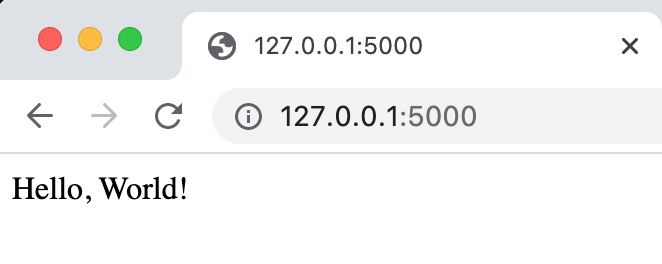
\includegraphics{images/helloworld.png}
\shorthandoff{=}
\caption{Hello world!}
\end{figure}

Sonrasında terminalde \texttt{CTRL+C} tuşları ile sunucunun sonlanması sağlanır. 


\section{About...}

Şimdi \url{http://127.0.0.1:5000/about} gibi bir sayfanın oluşmasını sağlayalım. Python'da bu şekilde bir çağrının gerçekleşmesini sağlayacak bir yönlendirici yazmamız gerekiyor. Aşağıda \texttt{decorator} ve \texttt{function} bu işi sağlayacak:


\begin{lstlisting}[style=mystyle]
@app.route("/about")
def about_page():
    return "This page is written in Python"
\end{lstlisting}

Böylece tüm Python dosyası aşağıdaki gibi bir içeriğe sahip olmuş olacak:

\begin{lstlisting}[style=mystyle]
from flask import Flask

app = Flask("My First App")

@app.route('/')
def hello_world():
    return 'Hello, World!'


@app.route("/about")
def about_page():
    return "This page is written in Python"

app.run()
\end{lstlisting}

Programı terminalde 

\begin{verbatim}
$ python3 flaskexample.py
\end{verbatim}

ile tekrar çalıştıralım. About sayfası aşağıdaki gibi gezilebilir olacak:

\begin{figure}[H]
\shorthandoff{=}
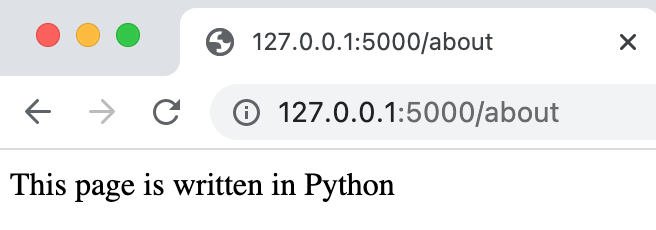
\includegraphics{images/about.png}
\shorthandoff{=}
\caption{About sayfası}
\end{figure} 



\section{Request parametreleri}

\begin{figure}[H]
\shorthandoff{=}
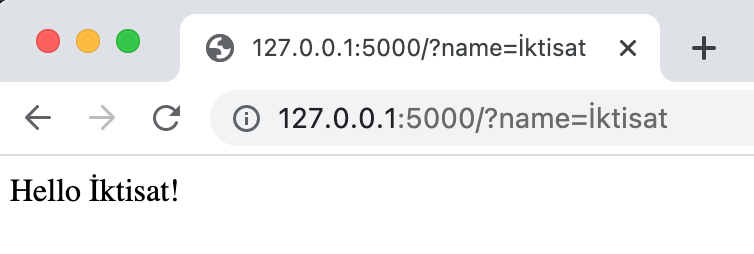
\includegraphics{images/requestparams.png}
\shorthandoff{=}
\caption{Request parametlerinin elde edilmesi}
\end{figure}

Sayfa URL'si içinde tanımlanan parametre ve değişkenleri Python'da elde edebilir ve değişen değerlere karşın farklı çıktının oluşmasını sağlayabiliriz. 

\begin{lstlisting}[style=mystyle]
from flask import Flask, request

app = Flask("My First App")

@app.route('/')
def hello_world():
    name = request.args.get("name")
    if name is None:
        return 'Hello, World!'
    else:
        return "Hello {}!".format(name)

app.run()
\end{lstlisting}


\section{HTML formları}

\begin{figure}[H]
    \shorthandoff{=}
    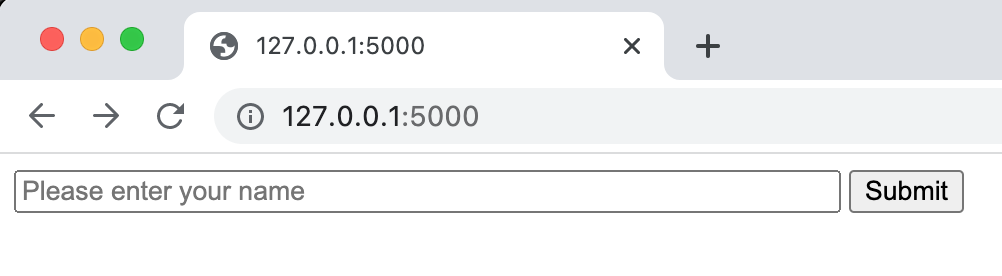
\includegraphics{images/emptyform.png}
    \shorthandoff{=}
    \caption{Boş form}
\end{figure}

\begin{figure}[H]
    \shorthandoff{=}
    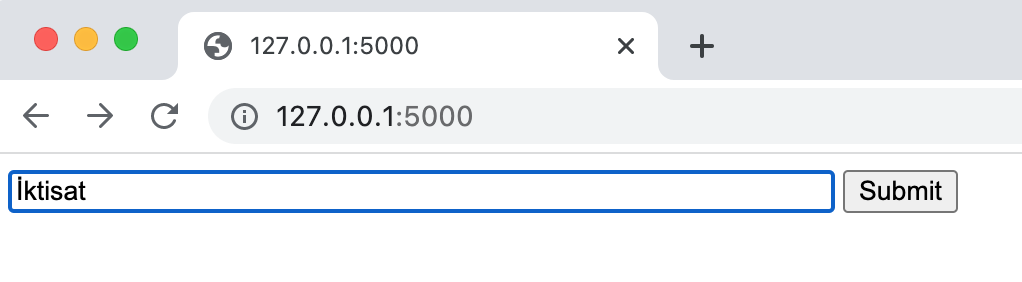
\includegraphics{images/formfilled.png}
    \shorthandoff{=}
    \caption{Dolu form}
\end{figure}


\begin{figure}[H]
    \shorthandoff{=}
    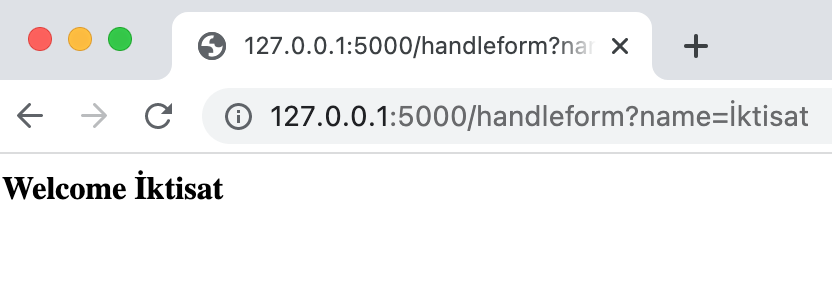
\includegraphics{images/welcomeiktisat.png}
    \shorthandoff{=}
    \caption{Submit işlemi sonrasında oluşan sayfa}
\end{figure}


\begin{figure}[H]
    \shorthandoff{=}
    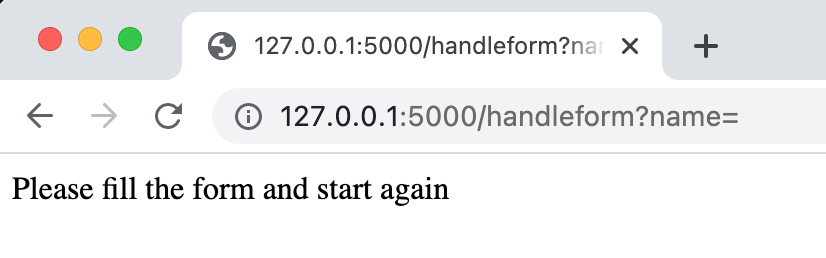
\includegraphics{images/pleasefilltheform.png}
    \shorthandoff{=}
    \caption{Metin kutusunun boş bırakıldığı durum}
\end{figure}


\pagebreak
\begin{lstlisting}[style=mystyle]
from flask import Flask, request

app = Flask("My First App")

@app.route('/')
def hello_world():
    content = """
    <form action="/handleform">
    <input type="text" 
    name="name" 
    size = 60
    placeholder="Please enter your name"/>
    <input type="submit">
    </form>
    """
    return content 

@app.route('/handleform')
def handle_form():
    name = request.args.get("name")
    if len(name) > 0:
        return "<b>Welcome {}</b>".format(name)
    else:
        return "Please fill the form and start again"

app.run()
\end{lstlisting}

\section{render template}

\texttt{index.html} templates adlı klasörde yer alsın ve içeriği aşağıdaki gibi olsun:

\begin{lstlisting}[style=mystyle]
<html>
<body>

A messege from Python:  
<b>
{{ msg }}
</b> 

</body>
</html>
\end{lstlisting}


Aşağıdaki gibi Python içinden bazı değer ve nesneler HTML sayfasında yer alacak şekilde transfer edilebilir:

\begin{lstlisting}[style=mystyle]
from flask import Flask
from flask.globals import request
from flask import render_template

app = Flask("My Application")

@app.route("/")
def index():
    return render_template("index.html", msg = "Hello world!")

app.run()
\end{lstlisting}

\begin{figure}[H]
    \shorthandoff{=}
    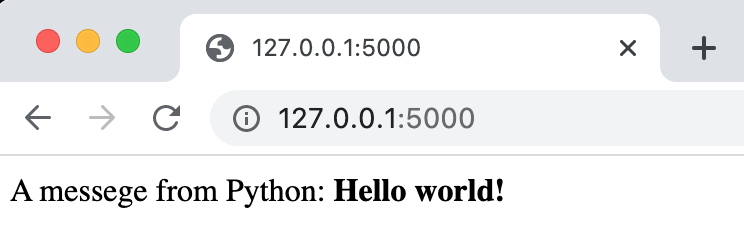
\includegraphics{images/templaterender.png}
    \shorthandoff{=}
    \caption{Template Rendering}
\end{figure}

\end{document}

